\chapter{Thermodynamics}

\begin{marginfigure}%
  \includegraphics[width=\linewidth]{entrope.jpg}
  \caption{Entropy is the monster of time}
  \label{fig:marginfig}
\end{marginfigure}


\textit{Only entropy comes easy.}  \\
\noindent\textbf{-   Anton Chekov}

\

\marginnote{

\begin{description}
\item[Thermodynamics] 
Thermodynamics is the branch of physics concerned with heat and temperature and their relation to energy and work.  It describes macroscopic variables of systems which are subject to general constraints, common to all materials, expressed in the four laws of thermodynamics.

\item[Heat]
Heat is energy that is transferred between a system and its surroundings, apart from work or or mass transfer.  When there is a suitable physical pathway, heat flows from a hotter temperature to a colder temperature body.  The pathway can be direct, as in conduction and radiation, or indirect, as in convective circulation.
\item[Temperature]
Temperature is the degree or intensity of heat in a substance.  Abstractly, it may be considered a representation of the random activity in a system.  

\item[Celsius] Celsius is a unit of temperature.  One degree Celsius represents the temperature change of one gram of water when $2.39\times10^{-5}\text{Joules}$ of heat is added to it.  It is offset so that the triple point of water is at zero degrees.

\item[Kelvin] Kelvin is a unit of temperature equivalent to Celsius except that its offset is such that the triple point of water is at 273.15 degrees.

\item[Thermal Equilibrium]
Thermal equilibrium is a condition where two substances in physical contact with each other exchange no net heat energy.  Substances in thermal equilibrium are at the same temperature.
\end{description}
}
\section{Systems and States}

\newthought{A thermodynamic system can be defined} in terms of its macroscopic states. In this way, a thermodynamic system is a macroscopic physical object, explicitly specified in terms of macroscopic physical variables that describe its macroscopic properties. 
A thermodynamic system is not simply a physical system.  Rather, in general, indefinitely many different alternative physical systems with specific microscopic states comprise a given thermodynamic system, because in general a physical system has vastly many more detailed characteristics than are mentioned in a thermodynamic description.

For example a system of 1000 particles could be described thermodynamically by the average kinetic energy of the particles.  This would be a thermodynamic state variable.  The actual microscopic state of each of the 1000 particles, each position and velocity at any instant would not be fully determined by the macroscopic variable.  The relationship between macro states and micro states is important in statistical mechanics, an approach to thermodynamics.



\section{History}
\newthought{Historically, the field of thermodynamics} has been the progressive fusion of many different schools of thought.  

Sadi Carnot, the "father of thermodynamics", published Reflections on the Motive Power of Fire (1824), a discourse on heat, power, energy, and engine efficiency. The paper outlined the basic energetic relations between the Carnot engine, the Carnot cycle, and motive power. It marked the start of thermodynamics as a modern science.

The first and second laws of thermodynamics emerged simultaneously in the 1850s, primarily out of the works of William Rankine, Rudolf Clausius, and William Thomson (Lord Kelvin).

\begin{figure}%
\begin{tikzpicture}
\node[inner sep=0pt] (russell) at (0,0)
    {\includegraphics[width=.22\textwidth]{carnot.jpg}};
    \node at (0,2) [anchor = north]{\footnotesize Carnot};
\node[inner sep=0pt] (whitehead) at (3,0)
    {\includegraphics[width=.22\textwidth]{thomson.jpg}};
     \node at (3,2) [anchor = north]{\footnotesize Kelvin};
    \node[inner sep=0pt] (whitehead) at (6,0)
    {\includegraphics[width=.22\textwidth]{clausius.jpg}};
     \node at (6,2) [anchor = north]{\footnotesize Clausius};
    \node[inner sep=0pt] (whitehead) at (9,0)
    {\includegraphics[width=.22\textwidth]{maxwell.jpg}};
     \node at (9,2) [anchor = north]{\footnotesize Maxwell};
      \node[inner sep=0pt] (whitehead) at (0,-4)
    {\includegraphics[width=.22\textwidth]{boltzmann.jpg}};
     \node at (0,-2) [anchor = north]{\footnotesize Boltzmann};
    \node[inner sep=0pt] (whitehead) at (3,-4)
    {\includegraphics[width=.22\textwidth]{gibbs.jpg}};
     \node at (3,-2) [anchor = north]{\footnotesize Gibbs};
      \node[inner sep=0pt] (whitehead) at (6,-4)
    {\includegraphics[width=.22\textwidth]{zeuner.jpg}};
     \node at (6,-2) [anchor = north]{\footnotesize Zeuner};
      \node[inner sep=0pt] (whitehead) at (9,-4)
    {\includegraphics[width=.22\textwidth]{waals.jpg}};
     \node at (9,-2) [anchor = north]{\footnotesize van der Waals};
%\draw[<->,thick] (russell.south east) -- (whitehead.north west)
    %node[midway,fill=white] {Principia Mathematica};
\end{tikzpicture}
  \caption{Many founders of thermodynamics have beards}
  \label{fig:marginfig}
\end{figure}


The foundations of statistical thermodynamics were set out by physicists such as James Clerk Maxwell, Ludwig Boltzmann, Max Planck, Rudolf Clausius and J. Willard Gibbs.  It provided a theoretical explanation for  classical thermodynamics.

American mathematical physicist Josiah Willard Gibbs showed how thermodynamic processes could include chemical reactions. By studying the energy, entropy, volume, chemical potential, temperature and pressure of the thermodynamic system, one can determine whether a chemical process would occur spontaneously.

\marginnote[-150pt]{
\section{Laws of Thermodynamics}
\begin{description}
\item[Zeroth Law]  If two systems are in thermal equilibrium respectively with a third system, they must be in thermal equilibrium with each other. This law helps define the notion of temperature.
\item[First Law]  When energy passes, as work, as heat, or with matter, into or out from a system, its internal energy changes in accord with the law of conservation of energy. Equivalently, perpetual motion machines of the first kind are impossible.
\item[Second Law]  In a natural thermodynamic process, the sum of the entropies of the interacting thermodynamic systems increases. Equivalently, perpetual motion machines of the second kind are impossible.
\item[Third Law]  The entropy of a system approaches zero as the temperature approaches absolute zero and is equal to the log of the multiplicity of the quantum ground states.
\end{description}}




\section {Zeroth Law}
Two systems are said to be in the relation of thermal equilibrium if they are linked by a wall permeable only to heat, and do not change over time.  Thermal equilibrium is transitive.  If two systems are in thermal equilibrium with a third system, then they are in thermal equilibrium with each other.   Systems at thermal equilibrium are at the same temperature.


\newpage

\section {Thermal Expansion}

\marginnote{
$$\alpha=\frac{1}{L_0}\frac{\Delta L}{\Delta T} $$
\vspace{10pt}
$$\beta=\frac{1}{V_0}\frac{\Delta V}{\Delta T} $$}

\newthought{Thermal expansion} is the tendency of matter to change in shape, area, and volume in response to a change in temperature, through heat transfer.  When a substance is heated, the kinetic energy of its molecules increases and maintain a greater average separation.  The fractional expansion divided by the change in temperature is called the material's coefficient of thermal expansion and generally varies with temperature.
            
\begin{margintable}[50pt]\index{typefaces!sizes}
  \footnotesize%
  \begin{center}
    \begin{tabular}{lr}
      \toprule
     Material & Linear Coefficient $\alpha$\\
      \midrule
    Aluminum    & 23.1 $\nicefrac{\mu}{\text{K}}$  \\
    Brass      & 19 $\nicefrac{\mu}{\text{K}}$  \\
    Carbon Steel      & 10.8 $\nicefrac{\mu}{\text{K}}$  \\
     Concrete   & 12 $\nicefrac{\mu}{\text{K}}$  \\
    Copper    & 17 $\nicefrac{\mu}{\text{K}}$  \\
    Iron    & 11.8 $\nicefrac{\mu}{\text{K}}$  \\
   Lead      & 29 $\nicefrac{\mu}{\text{K}}$  \\
    Mercury     & 61 $\nicefrac{\mu}{\text{K}}$  \\
    PVC    & 52 $\nicefrac{\mu}{\text{K}}$  \\
    Water     & 69 $\nicefrac{\mu}{\text{K}}$  \\
      \bottomrule
    \end{tabular}
  \end{center}
  \caption{Coefficients of linear expansion for various materials at $20{}^\circ\text{C}$.}
  \label{tab:font-sizes}
\end{margintable}
           
            
\subsection{Linear Expansion}
The change in the length of some object is the product of the original length, $L_0$, the change in temperature, $\Delta T$, and the coefficient of linear expansion, $\alpha$.
$$\Delta L=\alpha L_0 \ \Delta T $$
The coefficient of linear expansion is an intensive property of the material and changes with temperature.  It can even be negative for exotic materials.
\subsection{Volumetric Expansion}



Volumetric expansion is more appropriate for liquids and gases.  
$$\Delta V=\beta V_0 \ \Delta T $$
The coefficient of volumetric expansion is three times the coefficient of linear expansion.
$$\beta=3\alpha$$

\marginnote[-30pt]{The small calorie or gram calorie is the approximate amount of energy needed to raise the temperature of one gram of water by one degree Celsius at a pressure of one atmosphere.
\vspace{10pt}

$$1 \text{cal}\equiv 4.184 \text{J}$$}

\vspace{1cm}

\section{Specific Heat Capacity}

\begin{margintable}[10pt]\index{typefaces!sizes}
  \footnotesize%
  \begin{center}
    \begin{tabular}{lr}
      \toprule
     Material & Specific Heat\\
      \midrule
      Air     & 1.0 $\nicefrac{\text{kJ}}{\text{kg}\cdot\text{K}}$  \\
    Aluminum    & 0.087 $\nicefrac{\text{kJ}}{\text{kg}\cdot\text{K}}$  \\
    Argon     & 0.520 $\nicefrac{\text{kJ}}{\text{kg}\cdot\text{K}}$  \\
     Concrete   & 0.880  $\nicefrac{\text{kJ}}{\text{kg}\cdot\text{K}}$  \\
    Copper    & 0.385 $\nicefrac{\text{kJ}}{\text{kg}\cdot\text{K}}$  \\
    Iron    & 0.450 $\nicefrac{\text{kJ}}{\text{kg}\cdot\text{K}}$  \\
   Lead      & 0.129 $\nicefrac{\text{kJ}}{\text{kg}\cdot\text{K}}$  \\
    Mercury     & 0.140 $\nicefrac{\text{kJ}}{\text{kg}\cdot\text{K}}$  \\
    Water - Ice    & 2.05 $\nicefrac{\text{kJ}}{\text{kg}\cdot\text{K}}$  \\
    Water - Liquid     & 4.184 $\nicefrac{\text{kJ}}{\text{kg}\cdot\text{K}}$  \\
    Water - Vapor     & 2.00 $\nicefrac{\text{kJ}}{\text{kg}\cdot\text{K}}$  \\
      \bottomrule
    \end{tabular}
  \end{center}
  \caption{Specific heat capacities}
  \label{tab:font-sizes}
\end{margintable}
\newthought{Heat capacity} or thermal capacity is a measurable physical quantity equal to the ratio of the heat added to an object to the resulting temperature change.  The specific heat capacity is the heat capacity per unit mass of a material.  It is often referred to as the specific heat.
$$Q=mC \Delta T$$
$Q$ is the heat added to the system, $m$ is the mass, $C$ is the specific heat capacity and  $\Delta T$ is the change in temperature.
%$$Q=m\int _{T_i}^{T_f}c(T)\  dT$$

\newpage

\section{Latent Heat}
\begin{margintable}[0pt]\index{typefaces!sizes}
  \footnotesize%
  \begin{center}
    \begin{tabular}{lrr}
      \toprule
     Material & $L_{fusion}$&$L_{vapor}$ \\
      \midrule
    Ammonia    &  332 $\nicefrac{\text{kJ}}{\text{kg}}$ &  1369 $\nicefrac{\text{kJ}}{\text{kg}}$  \\
 Carbon Dioxide      &  184 $\nicefrac{\text{kJ}}{\text{kg}}$ &  574 $\nicefrac{\text{kJ}}{\text{kg}}$  \\
    Ethanol   &  108 $\nicefrac{\text{kJ}}{\text{kg}}$ &  855 $\nicefrac{\text{kJ}}{\text{kg}}$  \\
     Hydrogen   &  58 $\nicefrac{\text{kJ}}{\text{kg}}$ & 455 $\nicefrac{\text{kJ}}{\text{kg}}$ \\
   Lead      &  23.0 $\nicefrac{\text{kJ}}{\text{kg}}$&  871 $\nicefrac{\text{kJ}}{\text{kg}}$  \\
    Nitrogen    &  25.7 $\nicefrac{\text{kJ}}{\text{kg}}$&  200 $\nicefrac{\text{kJ}}{\text{kg}}$  \\
    Oxygen    &  13.9 $\nicefrac{\text{kJ}}{\text{kg}}$&  213 $\nicefrac{\text{kJ}}{\text{kg}}$  \\
    Water     &  334 $\nicefrac{\text{kJ}}{\text{kg}}$&  2265 $\nicefrac{\text{kJ}}{\text{kg}}$ \\
      \bottomrule
    \end{tabular}
  \end{center}
  \caption{Latent heats of fusion and vaporization}
  \label{tab:font-sizes}
\end{margintable}

Latent heat is energy released or absorbed, by a body or a thermodynamic system, during a constant-temperature process that is specified in some way. An example is latent heat of fusion for a phase change, melting, at a specified temperature and pressure.

The term was introduced around 1762 by Scottish chemist Joseph Black. It is derived from the Latin \textit{latere} (to lie hidden). Black used the term in the context of calorimetry where a heat transfer caused a volume change while the thermodynamic system's temperature was constant.

$$Q=mL$$

$Q$ is the heat added in the phase change, $m$ is the mass of the material and $L$ is the latent heat.



\section {Ideal Gas}
\begin{marginfigure}[50pt]
  \includegraphics[width=\linewidth]{pvt.jpg}
  \caption{Ideal gas dimensions of pressure, volume and temperature}
  \label{fig:marginfig}
\end{marginfigure}


\marginnote[0pt]{
\newthought{In statistical mechanics} the following molecular equation is derived from first principles.  It is another form of the ideal gas law.  
$$PV=Nk_BT$$
Here $N$ represents the number of particles and $k_B$ is the Boltzmann constant. 
$$k_B=1.38\times 10^{-23} \ \frac{\text{J}}{\text{K}}$$
Taking the two forms of the ideal gas law allows the relation between the gas constant and Boltzmann constant.
$$R=k_B N_A$$
Their ratio is Avogado's number, the number of particles in a mol.
$$N_A=6.02\times10^{23} \frac{1}{\text{mol}}$$
}

An ideal gas is a theoretical gas composed of many randomly moving point particles that do not interact except when they collide elastically. The ideal gas concept is useful because it obeys the ideal gas law, a simplified equation of state, and is amenable to analysis under statistical mechanics. One mole of an ideal gas has a volume of 22.7 L at STP as defined by IUPAC.

At normal conditions such as standard temperature and pressure, most real gases behave qualitatively like an ideal gas. Many gases such as nitrogen, oxygen, hydrogen, noble gases, and some heavier gases like carbon dioxide can be treated like ideal gases within reasonable tolerances.

\subsection{Ideal Gas Law}
The ideal gas law is the equation of state of a hypothetical ideal gas. It is a good approximation to the behavior of many gases under many conditions, although it has several limitations. It was first stated by Emile Clapeyron in 1834 as a combination of Boyle's law, Charles's law and Avogadro's Law.

$$PV=nRT$$

Here $P$ is the pressure, $V$ is the volume, $n$ is the number of moles of gas, $R$ is the gas constant and $T$ is the temperature.

$$R=8.31 \ \frac{\text{J}}{\text{mol}\cdot \text{K}}$$

\newpage

\subsection{Coefficient of Volumetric Expansion}
Beginning with the molecular ideal gas law, the coefficient of volumetric expansion $\beta$, may be derived.
$$PV=Nk_BT$$
The coefficient of thermal expansion is defined.
$$\beta=\frac{1}{V_0}\frac{\Delta V}{\Delta T} $$
Use of the ideal gas law yields the derived coefficient $\beta$.
$$\beta=\frac{N}{V_0}\frac{k_B}{P} $$

\subsection{Kinetic Theory}
\marginnote[-230pt]{
\subsection{Internal Energy}
The punchline of kinetic theory's model of the monatomic ideal is more than a model for pressure.  Kinetic theory gives the insight that the product of pressure and volume is proportional to the kinetic energy of the particles.
$$PV=\frac{2}{3}N \braket{KE}_{particle}=\frac{2}{3} \braket{KE}_{system}$$
Combine this with the molecular form of the ideal gas law.
$$PV=Nk_BT$$
This reveals the relationship between temperature and internal kinetic energy.
$$k_BT=\frac{2}{3} \braket{KE}_{particle}$$
Writing the total internal kinetic energy of the system $U$ yields the following.
$$U=\frac{3}{2} N k_B T$$
Temperature is a measure of the internal kinetic energy of a system. 

\subsection{Specific Heat}
The specific heat capacity of an ideal gas may be derived directly.
$$C=\frac{1}{m}\frac{\Delta U}{\Delta T}=\frac{3}{2} \frac{N}{m} k_B$$
$$C=\frac{3}{2}\frac{ k_B}{m_{part}}$$}

\marginnote{
\subsection{Equipartition of Energy}
Each degree of freedom contributes, on the average, $\frac{k_BT}{2}$ of energy per molecule.  For a monatomic ideal gas there are three translational degrees of freedom.  For a diatomic ideal gas there are two degrees of rotational freedom and three degrees of translational freedom.
\subsection{Statistical Distributions}
Boltzmann 
$$N(E)=N_0e^{\frac{-E}{k_BT}}$$
Maxwell-Boltzmann
$$N_v=4\pi N \left(\frac{m}{2\pi k_b T}\right)^{3/2}v^2e^{\frac{-mv^2}{2k_BT}}$$}

This kinetic theory of a monatomic ideal gas develops the concept of pressure and temperature from the microscopic/molecular view and connects to the ideal gas law.

Consider a particle, mass $m$, in a three-dimensional cube with side length $L$.  In the x spatial dimension the particle would bounce back and forth at a speed equal to the magnitude of the x-component of the velocity, $v_x$.  The particle has a momentum component $p_x$.
 $$p_x=mv_x$$
 On interaction with the wall the particle undergoes an elastic collision and imparts an impulse to the wall equal to twice the magnitude of the momentum in the x direction.
 $$\Delta p=2mv_x$$
 The average force associated with the repeated collision of the particle is determined.
 $$\braket{F}=\frac{\Delta p}{\Delta t}=\frac{2mv_x}{\nicefrac{2L}{v_x}}=\frac{mv_x^2}{L}$$
 With this the pressure may be determined.  
 $$P=\frac{\braket{F}}{A}=\frac{mv_x^2}{L^3}=\frac{mv_x^2}{V}$$
 For particles moving isotropically there is no prefered direction in space and therefore $\braket{v_x^2}=\nicefrac{\braket{v^2}}{3}$.  This yields the following expression for $N$ particles.
 $$PV=\frac{2}{3}N\frac{mv^2}{2}=\frac{2}{3}N \braket{KE}$$





\newpage

\section{Work}
\begin{marginfigure}[0pt]%
  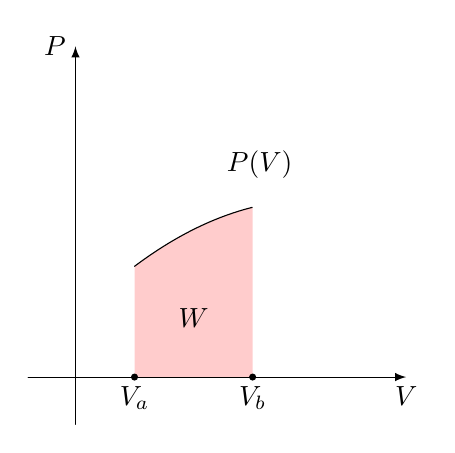
\begin{tikzpicture}
    [line cap=round,line join=round,x=2cm,y=2cm, scale=1.5, decoration={brace,amplitude=2pt}]
%main layer
%creating the ticks and xy-axis nodes
%some function
\fill[fill=red!20] (0.25,0) -- plot [domain=0.25:.75] (\x,{-\x^2/2+\x+0.25}) -- plot [domain=0.75: 0.25] (\x,0) -- cycle;

 \draw[smooth,samples=200,domain=0.25:0.75]
                                 plot(\x,{-\x^2/2+\x+0.25});
 

    \fill[black] (0.25,0) circle (0.3mm) node [anchor=north ,scale=1] {$ V_a$};
     \fill[black] (0.75,0) circle (0.3mm) node [anchor=north ,scale=1] {$V_b$};
      %  \fill[black] (0,0.25) circle (0.3mm) node [anchor=south east,scale=1] {\scriptsize$ v(0)$};

  \draw[-latex,color=black,thin] (-0.2,0) -- (1.4,0) node [anchor=north ,scale=1] {$V$};
   \draw[-latex,color=black,thin] (0,-0.2) -- (0,1.4)node [anchor=east ,scale=1] {$P$};
    \draw (0.6,0.8) node [anchor=south west ,scale=1] {$P(V)$};
        \draw (0.5,0.25) node [anchor=center ,scale=1] {$W$};
        
 \end{tikzpicture}
  \caption{Work is the area under the curve in a pressure versus volume graph.}
  \label{fig:marginfig}
\end{marginfigure}

Consider a gas in a piston chamber with cross sectional area $A$.  The work done by the gas, $W$ is the product of the force on the piston, $F$ and the displacement of the piston $\Delta x$.
$$W=F\Delta x=P A\Delta x=P \Delta V$$
The work done by an expanding gas is equal to the product of pressure and change in volume.  On a pressure vs temperature graph the work is the area under the line.
$$W=\text{Area}(P(V))$$


\section {Ideal Gas}
\begin{marginfigure}[50pt]
  \includegraphics[width=\linewidth]{piston.jpg}
  \caption{Piston chamber}
  \label{fig:marginfig}
\end{marginfigure}
\vspace{1cm}

\section{First Law of Thermodynamics}
The first law of thermodynamics is an energy conservation law.  The internal energy of a gas may be changed though the addition of energy by incoming heat $Q$ or removal or energy by the gas performing work on the surroundings $W$.
$$\Delta U=Q-W$$
For an ideal gas in a piston chamber the following is true.
$$PV=nRT=Nk_BT \hspace{2cm} W=\text{Area}(P(V))$$
Monatomic ideal gas:
$$U=\nicefrac{3}{2} PV$$
Diatomic ideal gas:
$$U=\nicefrac{5}{2} PV$$

\subsection{History}
The process of development of the first law of thermodynamics was by way of much investigative trial and error over a period of about half a century. The first full statements of the law came in 1850 from Rudolf Clausius and from William Rankine.  

Germain Hess in 1840 stated a conservation law for the so-called 'heat of reaction' for chemical reactions.  His law was later recognized as a consequence of the first law of thermodynamics, but Hess's statement was not explicitly concerned with the relation between energy exchanges by heat and work.

\newpage

\subsection{Isothermal Expansion}
\begin{marginfigure}[0pt]%
  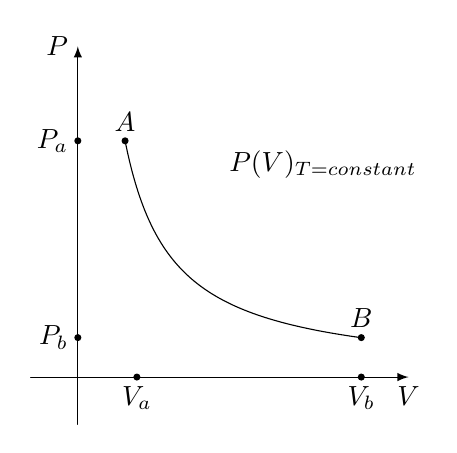
\begin{tikzpicture}
    [line cap=round,line join=round,x=2cm,y=2cm, scale=1.5, decoration={brace,amplitude=2pt}]
%main layer
%creating the ticks and xy-axis nodes
%some function

 \draw[smooth,samples=100,domain=0.2:1.2]
                             plot(\x,0.2/\x);

 
  \fill[black] (0.2,1) circle (0.3mm) node [anchor=south ,scale=1] {$ A$};
   \fill[black] (1.2,0.167) circle (0.3mm) node [anchor=south,scale=1] {$ B$};
 
 
 \fill[black] (0,1) circle (0.3mm) node [anchor=east ,scale=1] {$ P_a$};
     \fill[black] (0,0.167) circle (0.3mm) node [anchor=east ,scale=1] {$P_b$};

    \fill[black] (0.25,0) circle (0.3mm) node [anchor=north ,scale=1] {$ V_a$};
     \fill[black] (1.2,0) circle (0.3mm) node [anchor=north ,scale=1] {$V_b$};
      %  \fill[black] (0,0.25) circle (0.3mm) node [anchor=south east,scale=1] {\scriptsize$ v(0)$};

  \draw[-latex,color=black,thin] (-0.2,0) -- (1.4,0) node [anchor=north ,scale=1] {$V$};
   \draw[-latex,color=black,thin] (0,-0.2) -- (0,1.4)node [anchor=east ,scale=1] {$P$};
    \draw (0.6,0.8) node [anchor=south west ,scale=1] {$P(V)_{T=constant}$};
       % \draw (0.5,0.25) node [anchor=center ,scale=1] {$W$};
        
 \end{tikzpicture}
  \caption{Constant Temperature}
  \label{fig:marginfig}
\end{marginfigure}

During isothermal expansion temperature remains constant.
$$T=\text{constant}$$
Under these conditions pressure is inversely proportional to volume.
$$P(V)=\frac{Nk_BT}{V}$$
The work is the area under the $P(V)$ curve.
$$W=Nk_BT \ln \left( \frac{V_b}{V_a}\right)$$
The change in internal energy is given.
$$\Delta U=Q-Nk_BT \ln \left( \frac{V_b}{V_a}\right)$$



\subsection{Isobaric Expansion}
\begin{marginfigure}[70pt]%
  \begin{tikzpicture}
    [line cap=round,line join=round,x=2cm,y=2cm, scale=1.5, decoration={brace,amplitude=2pt}]

\draw[->,color=black,thick] (0.2,1) -- (0.7,1);
\draw[color=black,thick] (0.7,1) -- (1.2,1);
% \draw[->-,color=black,thin] (0.2,1) -- (1.2,1) node [anchor=north ,scale=1] {$V$};


 
  \fill[black] (0.2,1) circle (0.3mm) node [anchor=south ,scale=1] {$ A$};
   \fill[black] (1.2,1) circle (0.3mm) node [anchor=south,scale=1] {$ B$};
 
 
 \fill[black] (0,1) circle (0.3mm) node [anchor=east ,scale=1] {$ P_{a,b}$};
   
    \fill[black] (0.25,0) circle (0.3mm) node [anchor=north ,scale=1] {$ V_a$};
     \fill[black] (1.2,0) circle (0.3mm) node [anchor=north ,scale=1] {$V_b$};
      %  \fill[black] (0,0.25) circle (0.3mm) node [anchor=south east,scale=1] {\scriptsize$ v(0)$};

  \draw[-latex,color=black,thin] (-0.2,0) -- (1.4,0) node [anchor=north ,scale=1] {$V$};
   \draw[-latex,color=black,thin] (0,-0.2) -- (0,1.4)node [anchor=east ,scale=1] {$P$};
    \draw (0.6,0.5) node [anchor=south west ,scale=1] {$P(V)=constant$};
       % \draw (0.5,0.25) node [anchor=center ,scale=1] {$W$};
        
 \end{tikzpicture}
  \caption{Constant Pressure}
  \label{fig:marginfig}
\end{marginfigure}

During isobaric expansion pressure is constant.
$$P=\text{constant} $$
Work is easily computed.
$$ W=P \ \Delta V$$
The change in the internal energy given.
$$\Delta U=Q-P\Delta V$$


\subsection{Isovolumetric Cooling}
\begin{marginfigure}[30pt]%
  \begin{tikzpicture}
    [line cap=round,line join=round,x=2cm,y=2cm, scale=1.5, decoration={brace,amplitude=2pt}]
%main layer
%creating the ticks and xy-axis nodes
%some function


\draw[->,color=black,thick] (0.2,1) -- (0.2,0.6);
\draw[color=black,thick] (0.2,0.6) -- (0.2,0.2);
% \draw[->-,color=black,thin] (0.2,1) -- (1.2,1) node [anchor=north ,scale=1] {$V$};


 
  \fill[black] (0.2,1) circle (0.3mm) node [anchor=south ,scale=1] {$ A$};
   \fill[black] (0.2,0.2) circle (0.3mm) node [anchor=north,scale=1] {$ B$};
 
 
 \fill[black] (0,1) circle (0.3mm) node [anchor=east ,scale=1] {$ P_a$};
 \fill[black] (0,0.2) circle (0.3mm) node [anchor=east ,scale=1] {$ P_b$};
   
    \fill[black] (0.2,0) circle (0.3mm) node [anchor=north ,scale=1] {$ V_{a,b}$};
   
      %  \fill[black] (0,0.25) circle (0.3mm) node [anchor=south east,scale=1] {\scriptsize$ v(0)$};

  \draw[-latex,color=black,thin] (-0.2,0) -- (1.4,0) node [anchor=north ,scale=1] {$V$};
   \draw[-latex,color=black,thin] (0,-0.2) -- (0,1.4)node [anchor=east ,scale=1] {$P$};
    \draw (0.6,0.5) node [anchor=south west ,scale=1] {$V=constant$};
       % \draw (0.5,0.25) node [anchor=center ,scale=1] {$W$};
        
 \end{tikzpicture}
  \caption{Constant Volume}
  \label{fig:marginfig}
\end{marginfigure}

During isovolumetric heating the volume is constant.
$$V=\text{constant} $$
Therefore there is no work.
$$W=0$$
This makes the change in internal energy equal to the heat added to the system.
$$\Delta U=Q$$

\subsection{Adiabatic Expansion}
In an adiabatic process there is not heat transferred.
$$Q=0$$
Energy is transferred only as work.
$$\Delta U=-W$$

%\section{Heat Transfer}
%\subsection{Conduction}
%$$H=-kA\frac{dT}{dx}$$
%\subsection{Radiation: Stefan's Law}
%$$P=\sigma A e T^4$$
%$$ e=\text{emissivity} \hspace{2cm} \sigma=5.6696\times 10^{-8} \frac{\text{W}}{\text{m}^2\text{K}^4}$$
%\subsection{Convection}
%In convection the heated substance moves.

\newpage

\section{Heat Engines}
\begin{marginfigure}[0pt]
  \includegraphics[width=0.75\linewidth]{heat_engine.jpg}
  \caption{Heat engine}
  \label{fig:marginfig}
\end{marginfigure}

Work is done by heat transfer from a hot reservoir to a cold reservoir.

$$\text{Hot reservoir}\ \ \ Q_{in}=Q_h \hspace{2cm} \text{Cold reservoir}\ \ \ Q_{out}=Q_c$$ 
$$Q_{in}>Q_{out}$$
$$W=Q_{in}-Q_{out} \hspace{2cm} W>0$$
Work done by the engine is positive.  The engine is a source of power.
\subsection{Efficiency}
$$e=\frac{W}{Q_{in}}=\frac{Q_{in}-Q_{out}}{Q_{in}}$$
\section{Refrigerator}
\begin{marginfigure}[50pt]
  \includegraphics[width=0.75\linewidth]{refrig.jpg}
  \caption{Refrigerator}
  \label{fig:marginfig}
\end{marginfigure}
Heat is pushed against its temperature gradient from a cold reservoir to a hot reservoir.  
$$\text{Cold reservoir}\ \ \ Q_{in}=Q_c \hspace{2cm} \text{Hot reservoir}\ \ \ Q_{out}=Q_h$$ 
$$Q_{in}>Q_{out}$$
$$W=Q_{in}-Q_{out} \hspace{2cm} W<0$$
Work done by the refrigerator is negative.  Work is done on the refrigerator to increase the temperature gradient.  It requires a source of power.

 \section{Entropy}
 $S$ is the entropy of a system.  For reversible processes:
 $$T=\lim_{\Delta \rightarrow 0} \frac{\Delta Q}{\Delta S}$$
 $$\Delta Q=T \Delta S$$

 Isolated systems tend toward disorder.  Entropy is a measure of this disorder.  The entropy of the universe increases with every \textbf{irreversible} process.


\section{Second Law of Thermodynamics}
Entropy of the universe always stays the same or increases in any thermodynamic process.
\subsection{Kelvin-Plank}
It is \textbf{impossible} to construct a heat engine that, in a cycle, operates to absorb heat $Q_{in}$ and produce an equivalent amount of work, $W=Q_{in}$ so that $Q_{out}=0$.
\subsection{Clausius}
It is \textbf{impossible} to construct a refrigerator that, in a cycle, operates to absorb heat $Q_{in}$ from a cold sink and deliver it to a hot sink, $Q_{out}=Q_{in}$ so that $W=0$.


\section{The Carnot Engine}

\begin{marginfigure}[0pt]
  \includegraphics[width=\linewidth]{carnot_cycle.jpg}
  \caption{Carnot cycle}
  \label{fig:marginfig}
\end{marginfigure}

The Carnot engine is an idealized reversible engine with the maximal efficiency possible between a given hot and cold reservoir. 
\begin{enumerate}
\item Isothermal expansion  (in contact with the heat reservoir, constant temperature)
\item Adiabatic expansion  (thermally isolated, constant entropy)
\item Isothermal compression  (in contact with cold reservoir, constant temperature)
\item Adiabatic compression  (thermally isolated, constant entropy)
\end{enumerate}

 \subsection{Carnot Efficiency}
 $$e_c=\frac{T_h-T_c}{T_h}$$
 

 \subsection{Ideal Gas Reversible Process}
 $$dQ_r=dU+PdV=nC_VdT+nRT\frac{dV}{V}$$
 $$\Delta S=\int_i^f\frac{dQ_r}{T}=nC_V \ln \frac{T_f}{T_i}+nR\ln \frac{V_f}{V_i}$$
 \section{Irreversible Processes}
 \subsection{Free Expansion}
 $$\Delta S=nR\ln \frac{V_f}{V_i}$$
 \subsection{Heat Conduction}
 $$\Delta S=\frac{Q}{T_c}-\frac{Q}{T_h} $$
 \subsection{Heat Transfer}
  $$\Delta S=m_1c_1\ln \frac{T_f}{T_1} + m_2c_2\ln \frac{T_f}{T_2}$$
  
  \section{Third Law of Thermodynamics}
  The third law of thermodynamics is sometimes stated as follows, regarding the properties of systems in equilibrium at absolute zero temperature:
  
  \vspace{1cm}

The entropy of a perfect crystal at absolute zero is exactly equal to zero.

  \vspace{1cm}
  
At absolute zero (zero kelvin), the system must be in a state with the minimum possible energy, and the above statement of the third law holds true provided that the perfect crystal has only one minimum energy state. Entropy is related to the number of accessible microstates, and for a system consisting of many particles, quantum mechanics indicates that there is only one unique state (called the ground state) with minimum energy.
  
  \section{Statistical Mechanics}
  $$P_\beta(\sigma) ={e^{-\beta H(\sigma)} \over Z_\beta} \hspace{2cm} \beta=\frac{1}{k_BT} \hspace{2cm}Z_\beta = \sum_\sigma e^{-\beta H(\sigma)}\hspace{2cm} S=k\ln \Omega$$
 
